%; whizzy chapter
% -initex iniptex -latex platex -format platex -bibtex jbibtex -fmt fmt
% $B0J>e(B whizzytex $B$r;HMQ$9$k>l9g$N@_Dj!#(B

%     Tokyo Debian Meeting resources
%     Copyright (C) 2011 Junichi Uekawa
%     Copyright (C) 2011 Nobuhiro Iwamatsu

%     This program is free software; you can redistribute it and/or modify
%     it under the terms of the GNU General Public License as published by
%     the Free Software Foundation; either version 2 of the License, or
%     (at your option) any later version.

%     This program is distributed in the hope that it will be useful,
%     but WITHOUT ANY WARRANTY; without even the implied warranty of
%     MERCHANTABILITY or FITNESS FOR A PARTICULAR PURPOSE.  See the
%     GNU General Public License for more details.

%     You should have received a copy of the GNU General Public License
%     along with this program; if not, write to the Free Software
%     Foundation, Inc., 51 Franklin St, Fifth Floor, Boston, MA  02110-1301 USA

%  preview (shell-command (concat "evince " (replace-regexp-in-string "tex$" "pdf"(buffer-file-name)) "&"))
% $B2hA|%U%!%$%k$r=hM}$9$k$?$a$K$O(Bebb$B$rMxMQ$7$F(Bboundingbox$B$r:n@.!#(B
%(shell-command "cd image201101; ebb *.png")

%%$B$3$3$+$i%X%C%@3+;O!#(B

\documentclass[mingoth,a4paper]{jsarticle}
\usepackage{monthlyreport}

% $BF|IU$rDj5A$9$k!"Kh7nJQ$o$j$^$9!#(B
\newcommand{\debmtgyear}{2011}
\newcommand{\debmtgmonth}{6}
\newcommand{\debmtgdate}{18}
% (+ (* (- 2011 2005) 12) 6 -1) started from zero
\newcommand{\debmtgnumber}{77}

\begin{document}

\begin{titlepage}
\thispagestyle{empty}
% $B%?%$%H%k%Z!<%8(B:$BJT=8I,MW$JItJ,$O:G=i$N%^%/%m$KHt$P$9$3$H(B

\vspace*{-2cm}
$BBh(B\debmtgnumber{}$B2s(B $BEl5~%(%j%"(B Debian $BJY6/2q;qNA(B\\
\hspace*{-2cm}
\includegraphics[width=210mm]{image201003/debsen.eps}\\
\hfill{}\debmtgyear{}$BG/(B\debmtgmonth{}$B7n(B\debmtgdate{}$BF|(B

% $B$3$3$O%"%C%W%G!<%H$9$k$3$H(B
\rotatebox{10}{\fontsize{32}{32} {\gt $BFC=8(B1: Debian$B$G(BXSLT$B$r;H$C$F$_$?(B}}

\rotatebox{10}{\fontsize{32}{32} {\gt $BFC=8(B2: Sphinx$B$H(BDoxygen$B$r;H$C$F$_$?(B}}

\vspace*{-2cm}
\hfill{}
\includegraphics[height=6cm]{image200502/openlogo-nd.eps}
\end{titlepage}

\dancersection{Introduction}{$B>e@n(B $B=c0l(B}

\begin{multicols}{2}
 

 $B:#7n$N(BDebian$BJY6/2q$X$h$&$3$=!#$3$l$+$i(BDebian$B$N@$3&$K$"$7$rF'$_F~$l$k$H(B
 $B$$$&J}$b!"$9$G$K$I$C$W$j$H$D$+$C$F$$$k$H$$$&J}$b!"7n$K0l2s(BDebian$B$K$D$$(B
 $B$F8l$j$^$;$s$+!)(B

 Debian$BJY6/2q$NL\E*$O2<5-$G$9!#(B

 \begin{itemize}
 \item \underline{Debian Developer} ($B3+H/<T(B)$B$N0i@.!#(B
 \item $BF|K\8l$G$N!V(B\underline{$B3+H/$K4X$9$k>pJs(B}$B!W$r@0M}$7$F$^$H$a!"%"%C%W%G!<%H$9$k!#(B
 \item \underline{$B>l(B}$B$NDs6!!#(B
 \begin{itemize}
  \item $BIaCJ$P$i$P$i$J>l=j$K$$$k?M!9$,(B face-to-face $B$G=P2q$($k>l$rDs6!(B
	$B$9$k!#(B
  \item Debian $B$N$?$a$K$J$k$3$H$r8l$k>l$rDs6!$9$k!#(B
  \item Debian$B$K$D$$$F8l$k>l$rDs6!$9$k!#(B
 \end{itemize}
 \end{itemize}		

 Debian$B$NJY6/2q$H$$$&$3$H$G5f6KE*$K$O;22C<TA40w$,(BDebian Package$B$r$,$j$,$j(B
 $B$H:n$k%9!<%Q!<%O%C%+!<$K$J$C$?;Q$rLQA[$7$F$$$^$9!#>pJs$N6&M-!&3hMQ$rDL$7(B
 $B$F(B Debian$B$N:#8e$NG=F0E*$JE83+$X$NEZBf$H$7$F!"!V>l!W$H$7$F$N6u4V$rDs6!$9(B
 $B$k$N$,L\E*$G$9!#(B

\end{multicols}

\newpage

\begin{minipage}[b]{0.2\hsize}
 \definecolor{titleback}{gray}{0.9}
 \colorbox{titleback}{\rotatebox{90}{\fontsize{80}{80} {\gt $B%G%S%"%sJY6/2q(B} }}
\end{minipage}
\begin{minipage}[b]{0.8\hsize}
\hrule
\vspace{2mm}
\hrule
\begin{multicols}{2}
\tableofcontents
\end{multicols}
\vspace{2mm}
\hrule
\end{minipage}

\dancersection{$B;vA02]Bj(B}{$B4d>>(B $B?.MN(B}

$B:#2s$N;vA02]Bj$O0J2<$G$9(B:
\begin{enumerate}
 \item $B:G6a(BDebian$B$G<+J,$,$d$C$?$3$H$d6=L#$N$"$k$3$H$r65$($F$/$@$5$$!#(B
\end{enumerate}
$B$3$N2]Bj$KBP$7$FDs=P$$$?$@$$$?FbMF$O0J2<$G$9!#(B
\begin{multicols}{2}
{\small
 
\begin{prework}{ やまだ }

最近新しいカーネルを自分でビルドすることが再び
増えてきたので、その周りでごそごそやってます。
\begin{enumerate}
\item gitでタグを打って
\item そのタグをバージョンにして
\item ビルドして
\item テストVMに導入して
\item ついでに配布サーバに設置
\end{enumerate}

の自動化とかやりました。

興味というか次に調べたいのは *-module-source な
カーネルモジュールパッケージの作り方とかDKMSの使い方。
普通のパッケージと違う点が多々ありそう。
\end{prework}

\begin{prework}{ 野首 }

ホームのMHフォルダを外から見れるようuw-imapdを入れました。インストールし
 てdebconfに答えるだけでSSL readyなimap環境になりました。
\end{prework}

\begin{prework}{ MATOHARA }

2010年11月の勉強会資料を見ながらnilfs2 をバックアップディスクに設定して
 みました.
リサイズ機能も来たようなので試してみたいです.
- [PATCH 0/4] nilfs2 resize support -- Linux NILFS Development
\url{http://www.spinics.net/lists/linux-nilfs/msg00869.html}
\end{prework}

\begin{prework}{ hattorin }

バングラデシュでDebianインストールして、ネットワークの監視系ツールをいろ
 いろとセットアップしてきました。今はDebian on SqueezeでTokyoTyrantの
 KeyValueを使い、特定の問題を早く計算するためにネットワークを使って計算
 を早くするような仕組み作りをしています。
\end{prework}

\begin{prework}{ キタハラ }

実家でプリンタの設定したり、
スキャナーの設定に失敗してました。

\end{prework}

\begin{prework}{ koedoyoshida }

最近Debianで自分がやったこと
\begin{itemize}
\item ようやく、メイン環境をSqueezeにupdate
wide-dhcpがupdateできずにはまったが、下記を見て解決。
\url{http://www.flcl.org/~takasugi/tdiary-org/?date=20061023}
\item OSC仙台に参加、出展。
\end{itemize}


\end{prework}

\begin{prework}{ emasaka }

sidでちょっとはまったとこについて、GitHubでupstreamに簡単なパッチをpull
 requestしたら、そのバージョンが数日後にsidに降りてきました。
\end{prework}

\begin{prework}{ dictoss(杉本 典充) }

最近やっていることはkfreebsdを常用していること、Debianを開発環境として
 gtkアプリを試作していること。
今後はkfreebsdでIS03を使ってテザリング、klinuxよりkfreebsdの方がおすすめ
 といえる有利分野を見つけることをやりたい。
\end{prework}

\begin{prework}{ なかおけいすけ }

興味があること:DebianLive
最近ネカフェで一夜を明かしたのですが、ネカフェのPCにコンパイラが入ってな
 くて困ったので、USBやSDカードにインストールしたDebianを持ち歩いていると
 ハッピーになれるのではないかと。
\end{prework}

\begin{prework}{ 吉野(yy\_y\_ja\_jp) }

バグレポートとDDTSS/DDTPぐらいでしょうか.
\end{prework}

\begin{prework}{ henrich }

いくつかパッケージやメッセージをルーティンの更新しました。

\end{prework}

\begin{prework}{ Osamu MATSUMOTO }

\begin{itemize}
\item インフラ,サーバ管理の自動化\\
 自動インストール,構成管理,コンフィグ投入, 監視のまでを
 ラフに綺麗に繋ぎたい。Debian的な良い組み合わせあったら教えてください。
 (cobbler+ puppet/cfengine+ nagios + なんかwebcgi的な)
\end{itemize}

\end{prework}

\begin{prework}{ まえだこうへい }
\begin{itemize}
\item *diagシリーズ(http://blockdiag.com/)のdebパッケージ化中。
\item さくらのVPSを先月契約して、lxc \& Squeezeで開発\&検証環境に。
\item あらきさんメンテナンスのDebianのAMI使ってAWSでごにょごにょと。
\end{itemize}
\end{prework}

\begin{prework}{ yamamoto }

\begin{itemize}
\item 最近Debianで自分がやったこと\\
ポチポチと公式パッケージのリビルドをしました。
\item 興味のあること\\
移植。
\end{itemize}

\end{prework}

\begin{prework}{ 岩松 信洋 }

\begin{itemize}
\item SH4 buildd のメンテ。
\item libpng15 の experimental へのアップロードとtransition作業。
\item スポンサーのパッケージチェック、アップロードなど。
\end{itemize}

\end{prework}

\begin{prework}{ 野島 貴英 }

\begin{itemize}

\item pythonでgnome-notifyめがけて再生中のデータのメタデータ送る「できるだ
 け簡単にできる」totemのプラグイン書いてみた。
 \url{http://d.hatena.ne.jp/nozzy123nozzy/20110502/1304322969}
\item sidのalsa-lib,alsa-utils,alsa-driverの解析中。
(bluetoothヘッドフォン出力相手に、alsaのみで、演奏中の音をcaptureしたい
 し、音が出る複数のアプリの音をmixして出力したいっ)
\item sidのlinux-image-2.6.39-2-686-paeにて、multi-stateなusb装置にejectコ
 マンド発行すると高い確率でOopsする件のデバッグを誰かがパッチ出すまでや
 り中。(いったい誰だ、dptぶっ壊すのは...)

\end{itemize}

\end{prework}

\begin{prework}{ 上川純一 }
\begin{itemize}
\item xslt のツールチェインをいろいろといじってみたり。
\item Javascript のコードを書いてみたり。
\end{itemize}
\end{prework}

}
\end{multicols}

\dancersection{$B:G6a$N(BDebian$B4XO"$N%_!<%F%#%s%0Js9p(B}{$B4d>>(B $B?.MN(B}
\subsection{$BEl5~%(%j%"(BDebian$BJY6/2q(B76$B2sL\Js9p(B}

$BEl5~%(%j%"(BDebian$BJY6/2q(B76$B2sL\$O?7Bg5WJ]1X(B
$B$N6a$/$K$"$k8M;3@8363X=,4[$G9T$$$^$7$?!#(B
$B>e@n$5$s$,(B apache2 $B$N%b%8%e!<%k$N:n@.$K$D$$$F$*OC$7$7!"(B
Debian $B$N(Bapache2$B%b%8%e!<%k:n@.$N$O$^$j$I$3$K$D$$$F@9$j>e$,$j$^$7$?!#(B\\
Nifty $B$5$s$,(BNifty Cloud $B$K(B Debian 
$B;H$($k$h$&$K$9$k$H$$$&$3$H$G!"$I$N$h$&$J%$%a!<%8$K$7$?$i$$$$$N$+!"$I$N$h$&$J%P%C%/%(%s%I$,I,MW$J$N$+5DO@$7$^$7$?!#(BNifty$B$5$s$G$=$m$=$m(BDebian$B$,;H$($k$h$&$K$J$C$F$$$k$H;W$$$^$9!J$?$V$s!K!#(B
$B4d>>$,(B Debian $B$G$N(B m68k $B3+H/$K$D$$$F$N>u67$HJ}K!$rOC$7$^$7$?!#(BDebian $B$G$O<B5!$O$"$^$j;H$o$l$F$*$i$:!"(BAranym$B$H$$$&%(%_%e%l!<%?>e$G3+H/$r9T$C$F$$$k$H$N$3$H!#(BDebian $B$G(B m68k $B$,:FEY%j%j!<%9$5$l$kF|$O$/$k$N$+3Z$7$_$G$9!#(B
$B;3K\$5$s$,(Bppc64$B%]!<%F%#%s%0$K$D$$$FJs9p$7$^$7$?!#A02s$N=IBj$G$O(B powerpcspe $B$H$N%Y%s%A%^!<%/$r<h$C$F$-$F!"(Bppc64$B$HHf$Y$F$I$N$h$&$J%a%j%C%H%G%a%j%C%H$,$"$k$N$+$r8+$F$_$h$&$H$$$&$3$H$G$7$?$,!"$J$<$+(Bppc$B$H$N%Y%s%A$r<h$C$F$-$?$N$G:FEY=IBj$K$J$j$^$7$?!#%Q%C%1!<%8$OB7$C$F$$$k$N$G2H$K(Bppc64$B%^%7%s$,L2$C$F$$$k?M$O;n$7$F$_$F$O$$$+$,$G$7$g$&$+!#(B


% (query-replace-regexp "<.*?>" "")
% (query-replace-regexp "^[	 ]\+" "")

\subsection{OSC 2011 Hokkaido $B=PD%(BDebian$BJY6/2qJs9p(B}
2011$BG/(B6$B7n(B11$BF|(B($BEZ(B)$B$KKL3$F;;%KZ;T$G%*!<%W%s%=!<%9%+%s%U%!%l%s%9(B2011$BKL3$F;$,3+:E$5$l$^$7$?!#(B

Debian$BJY6/2q$G$O%?%$%H%k!V(BDebian 6.0(squeeze) \& Debian Update$B!W$H$7$F:4!9LZMNJ?$5$s$,%;%C%7%g%s$r9T$$$^$7$?!#(B
$B%;%C%7%g%s$K$O(B14$BL>$,;22C$7!"<ALd$G$O%P%0Js9p$N<j=g$r3NG'$9$k<ALd$,=P$5$l$^$7$?!#(B


GPG$B%-!<%5%$%s%Q!<%F%#$N;22C<T$O%3!<%G%#%M!<%?!<$r4^$a$F(B3$BL>$G$"$j!"KL3$F;$NJ}!9$X(BGPG$B%-!<$N7<LX3hF0$r0z$-B3$-9T$C$F$$$/I,MW$,$"$j$=$&$G$9!#(B

\begin{center}
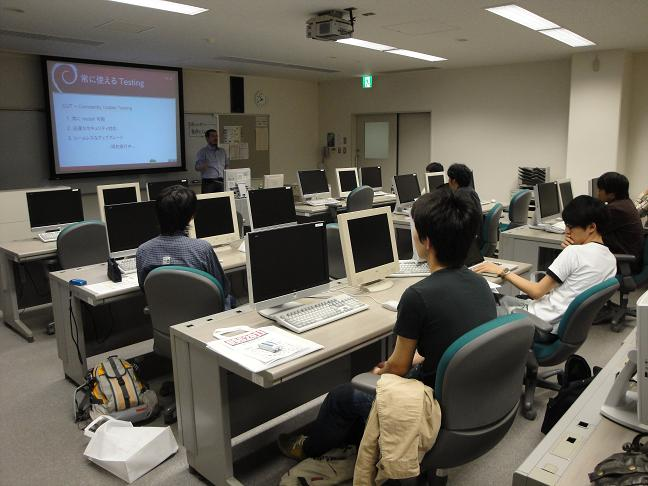
\includegraphics[width=10cm]{image201106/osc11do.jpg}
\end{center}

\subsection{OSC 2011 Sendai $B=PD%(BDebian$BJY6/2qJs9p(B}
2011$BG/(B5$B7n(B21$BF|(B($BEZ(B)$B$K5\>k8)@gBf;T$G%*!<%W%s%=!<%9%+%s%U%!%l%s%9(B2011$B@gBf$,3+:E$5$l$^$7$?!#(B

Debian$BJY6/2q$G$O5HED!wHD66$,E8<($G=PE8$7$^$7$?!#(B
\begin{enumerate}
\item$B!VEl5~%(%j%"(BDebian$BJY6/2q(B/$B4X@>(BDebian$BJY6/2q!W$N>R2p(B
\item$B!V$"$s$I$-$e$a$s$F$C$I$G$S$"$s(B(Debian$BJY6/2q;qNA$N%5%^%j(B)$B!W$NE8<(!"HNGd(B
\item$B!V(BDebian Squeeze$B$NE8<(!W6qBNE*$K$O!V(BDebian GNU/kFreeBSD$B!W$NE8<((B
\end{enumerate}
$B<g$K>e5-$r$*$3$J$$$^$7$?!#(B
$B%a%$%s%[!<%kF~$j8}@5LL$H$$$&G[CV$K$b7C$^$l!"B?$/$NJ}$KN)$A4s$C$FD:$-$^$7$?!#(B

\begin{center}
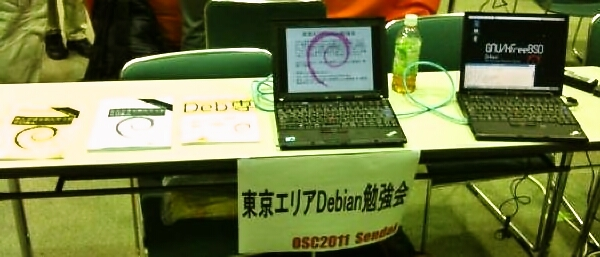
\includegraphics[width=10cm]{image201106/oscsendai.jpg}
\end{center}

\dancersection{Debian Trivia Quiz}{$B4d>>(B $B?.MN(B}

$B$H$3$m$G!"$_$J$5$s(B Debian $B4XO"$NOCBj$K$*$$$D$$$F$$$^$9$+!)(BDebian$B4XO"$NOC(B
$BBj$O%a!<%j%s%0%j%9%H$r$h$s$G$$$k$HDI@W$G$-$^$9!#$?$@$h$s$G$$$k$@$1$G$O$O(B
$B$j$"$$$,$J$$$N$G!"M}2rEY$N%F%9%H$r$7$^$9!#FC$K0l?M$@$1$G$O0UL#$,$o$+$i$J(B
$B$$$H$3$m$b$"$k$+$bCN$l$^$;$s!#$_$s$J$G0l=o$KFI$s$G$_$^$7$g$&!#(B

$B:#2s$N=PBjHO0O$O(B\url{debian-devel-announce@lists.deban.org} $B$d(B \url{debian-devel@lists.deban.org}$B$KEj9F$5$l$?(B
$BFbMF$H(BDebian Project News$B$+$i$G$9!#(B

\begin{multicols}{2}
 %; whizzy-master ../debianmeetingresume201101.tex
% $B0J>e$N@_Dj$r$7$F$$$k$?$a!"$3$N%U%!%$%k$G(B M-x whizzytex $B$9$k$H!"(Bwhizzytex$B$,MxMQ$G$-$^$9!#(B
%
% $B$A$J$_$K!"%/%$%:$OJL%V%i%s%A$G:n@.$7!"$N$A$K%^!<%8$7$^$9!#5U$K%^!<%8$7(B
% $B$J$$$h$&$K$7$^$7$g$&!#(B
% (shell-command "git checkout quiz-prepare")

\santaku
{alioth.debian.org$B$,(B2$BBf$KJ,$+$l$^$7$?!#$=$N%5!<%PL>$O!)(B}
{vasks.debian.org $B$H(B wagner.debian.org}
{volks.debian.org $B$H(B don.debian.org}
{dennys.debian.org $B$H(B gusto.debian.org}
{A}
{$B$[$+$O%U%!%_%l%9$NL>A0(B}

\santaku
{$B8=:_9T$o$l$F$$$k(BPerl transition $B$N(BPerl$B%P!<%8%g%s$O!)(B}
{5.12}
{5.13}
{5.14}
{A}
{5.14$B$O$^$@(Bexperimental$B$G$9!#(B}

\santaku
{$B%W%i%$%^%j%_%i!<%5!<%P$,?7$7$/DI2C$5$l$?9q$O!)(B}
{$B%A%e%K%8%"(B}
{$BCf9q(B}
{$B%^%@%,%9%+%k(B}
{B}
{$B%A%e%K%8%"$H%^%@%+%9%+%k$O%_%i!<!#%W%i%$%^%j$G$O$J$$!#(B}

\end{multicols}

%-------------------------------------------------------------------------------
\dancersection{Debian JP $BDjNc2q5D=hM}7O$K(BXSLT$B$r;H$C$F$_$?(B}{$B>e@n=c0l(B}
%-------------------------------------------------------------------------------
\index{xsltproc}

\subsection{$BGX7J(B}

Debian$BJY6/2q$N4k2h2q5D$O(BIRC$B$rCf?4$H$7$F(B2006$BG/$K3+;O$7!"(BDebian JP $B$NDjNc2q(B
$B5D$H$7$F:#$bB3$$$F$$$^$9!#Ev=i$O7hDj;v9`$J$I$K$D$$$F%F%-%9%H%U%!%$%k$G$^(B
$B$H$a$k$H$$$&7A$r$H$C$F$$$^$7$?!#(BIRC$B$G$h$j8zN($h$/5DO@$9$kJ}K!$rLO:w$7$?7k(B
$B2L!"5DO@$7$J$,$i5D;vO?$rJT=8$9$k$H$$$&%9%?%$%k$,3NN)$7!"$=$l$r;Y1g$9$k$?(B
$B$a$N%D!<%k$r@0Hw$7$^$7$?!#(B

$B5D;vO?$N%=!<%9$O5DD9$,(BXML$B$G5-=R$7$F!"5DO@$N:GCf$OHsF14|$K(BJavascript$B$GFb(B
$BMF$,99?7$5$l$k(BHTML$B%U%!%$%k$rMxMQ$7$^$9(B($B@$4V0lHL$G$O(BAJAX$BE*$H$G$b$h$V$h$&(B
$B$G$9(B)$B!#(B

IRC$B$G$NDjNc2q5D$N5DO@$NA0$H8e$K$O5D;v0F$H5D;vO?$r%a!<%j%s%0%j%9%H$K$*$/$C(B
$B$F$$$^$9!#%a!<%j%s%0%j%9%H$K%a!<%k$G$J$2$k:]$K$O!"%F%-%9%H%U%)!<%^%C%H$K(B
$B$7$FAw$C$F$$$^$9!#(B

$B$"$H!"8=:_MQES$,$J$$$G$9$,!"(B\LaTeX $B7PM3$G(BPDF$B7A<0$G$N=PNO$J$I$b%5%]!<%H$7(B
$B$F$$$^$9!#(B

$B8=:_$N<BAu$ONr;KE*$J7P0^$K$h$j(BXML$B$N=hM}7O$O(B dancer-xml $B%i%$%V%i%j$H(B
boost$B$rMxMQ$7$?(BC++$B$N%W%m%0%i%`$K$J$C$F$$$^$9!#(B
dancer-xml\cite{dancer-xml} $B$O(B10$BG/A0$K<c5$$N$$$?$j$G<BAu$7$?(BXML$BIwJ8=q$N%Q!<(B
$B%5!<$G$9!#0lIt%(%s%F%#%F%#!<$^$o$j$J$I??LLL\$K<BAu$7$F$$$J$$ItJ,$,$"$k$?(B
$B$a!"E,@Z$J=hM}$,$J$5$l$F$$$J$$$3$H$,$"$j$^$9$,!"KM$N9%$_$K6uGrJ8;z=hM}$O(B
$B%A%e!<%K%s%0$5$l$F$*$j2wE,$G$9!#(B

$B:#2s$ND)@o$O!"FH<+(BC++$B%3!<%I%Y!<%9$r(BXSLT$B$K$N$;BX$($F$_$k$H$$$&D)@o$G$9!#(B

\begin{figure}[ht]
 \begin{center}
  \includegraphics[width=0.5\hsize]{image201106/ircsystem.eps}
 \end{center}
\label{fig:ircsystem-general}\caption{IRC $B2q5D%7%9%F%`$N%G!<%?7A<0$N35MW(B}
\end{figure}

\subsection{XSLT$B$C$F$I$s$J8@8l(B?}

XSLT$B$O(BXML$B$G5-=R$9$k(BXML$B=hM}8@8l$G$9!#(B

XSLT$B5,3J$K$O(B1999$BG/$K:vDj$5$l$?(BXSLT 1.0 $B$H!"(B2007$BG/$4$m$N(BXSLT 2.0$B$,$"$j$^$9!#(B
$B:#2s$O<BAu$,==J,8O$l$F$$$k$H;W$o$l$k(B XSLT 1.0 $B$N=hM}7O$r:NMQ$7$^$7$?!#(B
XSLT2.0$B$N(BDebian$B$GMxMQ$G$-$k<BAu$H$7$F$O(B libsaxonb-java$B$,$"$k(B
$B$h$&$G$9$,!":#2s$OD4::$7$F$$$^$;$s!#(B

$B%W%m%0%i%`$r=q$/$H$-$K$9$Y$-J8=q$H$7$F$O!"(BXSLT$B<+BN$N(B1999$BG/$K:vDj$5$l$?5,(B
$B3J(B\cite{xslt1999}$B$H!"(BXSLT$B$NCf$G5-=R$G$-$k(BXPATH$B$N5,3J(B\cite{xpath1999}$B$r;2(B
$B>H$9$k$H$h$$$G$7$g$&!#(B

XSLT$B$@$1$G$O$"$^$j9bEY$J%W%m%0%i%_%s%0$O$G$-$J$$$s$8$c$J$$$+$H;W$o$l$k$+(B
$B$b$7$l$^$;$s$,!"4X?t7?8@8l$H$7$F==J,$J5!G=$rDs6!$G$-$kNO$O$"$k$h$&$G$9(B
\cite{fxslt2003}$B!#(B

\subsection{Debian $B$GMxMQ2DG=$J(B XSLT$B=hM}7O(B}

Debian$B$GI}9-$/;H$o$l$F$$$F0BDj$7$F$$$k$H$*$b$o$l$k$N$H!"4JC1$KMxMQ$G$-$k(B
$B$H$$$&M}M3$G=hM}7O$H$7$F(B xsltproc $B$r:NMQ$7$^$7$?!#(B

Debian $B$G$N(B xsltproc $B$N%$%s%9%H!<%k$O4JC1(B
\begin{commandline}
$ apt-get install xsltproc
\end{commandline}
%$

$B%3%^%s%I%i%$%s$G0J2<$N$h$&$K<B9T$9$k$HI8=`=PNO$K=hM}:Q$_(BXML$B$,=PNO$5$l$^$9!#(B

\begin{commandline}
$ xsltproc [$B%9%?%$%k%7!<%H(B] [$B=hM}$9$k(BXML$B%U%!%$%k(B]
\end{commandline}
%$

\subsection{$B6qBNNc(B:HTML}

$B$=$l$G$O!"(BHTML$B=PNO$N>l9g$r8+$F$_$^$7$g$&!#(B
\url{meetinglog:html.xsl}$B$G$9!#(B
XML$BJ8=q$+$i(BHTML$BJ8=q$r@8@.$9$k$K$O$=$l$J$j$KJXMx$J8@8l$G$9!#(B

$BA0H>$N%3!<%I$r$=$N$^$^7G:\$7$^$9!#(B
$B$3$l$O!"(BXML$B%I%-%e%a%s%HA4BN$K%^%C%A$9$k%k!<%k$r5-=R$7$O$8$a$k$^$G$NItJ,(B
$B$G$9!#(B
XML$BL>A06u4V$H$7$F!"%G%U%)%k%H$r(BHTML$B!"(Bxsl$B$r(Bxslt$B$NL>A06u4V$K3d$jEv$F$F$$$^(B
$B$9!#(B

xml:output $B$G=PNO7A<0$r(BHTML$B$H;XDj$9$k$3$H$G(BXML$B%X%C%@$,=PNO$5$l$:$KJXMx$G(B
$B$9!#(B

\begin{commandline}
<?xml version="1.0"?>
<!DOCTYPE xsl:stylesheet>
<xsl:stylesheet version="1.0"
  xmlns:xsl="http://www.w3.org/1999/XSL/Transform"
  xmlns="http://www.w3.org/1999/xhtml">
  <xsl:output method="html" />
  <xsl:template match="/">
    <html>
      <head>
\end{commandline}

$BB>$K(BXSLT$B$NFCD'E*$J$H$3$m$O!"(Bvalue-of$B!!$GCM$r$H$C$F$-$F$$$^$9!#(BXPATH
$B$N=q<0$G;XDj$7$F$$$^$9$,!"(B
\begin{commandline}
	<h1><xsl:value-of select="meetinglog/head/title"/></h1>
\end{commandline}

$B$O!"(BXML$BJ8=q$N0J2<$N$h$&$J%(%l%a%s%H$KF~$C$F$$$kCM$rCj=P$7$^$9!#(B
\begin{commandline}
 <meetinglog>
   <head>
     <title>$B%?%$%H%k(B</title>
   </head>
 </meetinglog> 
\end{commandline}

$B5D;vO?$N>l9g$N%a%$%s%k!<%W$O!"3F5D;v$KBP$7$F$N=hM}$G$9!#(B
xsl$B$N(Bxsl:for-each$B$r$D$+$$!"(BXML$B$N%(%l%a%s%H%N!<%I$N?t$@$1%k!<%W$7$^$9!#(B
HTML$B%?%0$O$=$N$^$^=PNO$5$l$^$9$,!"$b$7(BHTML$B$N%"%H%j%S%e!<%H$J$I$r(BXSLT$B$G@8(B
$B@.$7$?$$>l9g$O!"(Bxsl:element $B$r;H$C$F%(%l%a%s%H$r@8@.$7$^$9!#(B

position()$B4X?t$O8=:_$N%(%l%a%s%HHV9f$r$/$l$k$N$G$3$&$$$&>l9g$KJXMx$G$9!#(B

\begin{commandline}
           <xsl:for-each select="meetinglog/body">
	      <tr>
		<th>
		  <xsl:element name="a">
		    <xsl:attribute name="href">#gian<xsl:value-of select="position()" /></xsl:attribute>
		  </xsl:element>
		  $B5D0F(B<xsl:value-of select="position()" />
		</th>
		<td class="bodytitle">
		  <xsl:value-of select="./title" />
		</td>
 ....
 </xsl:for-each> 
\end{commandline}

\subsection{$B6qBNNc(B:Text$B=PNO(B}

Text$B=PNO$N>l9g$b$_$F$_$^$7$g$&!#(B
\url{meetinglog:txt.xsl}
$B%F%-%9%H=PNO$r$7$h$&$H$7$O$8$a$k$H<c436l$7$/$J$C$F$-$^$9!#$G$-$J$$$o$1$G(B
$B$O$J$$$N$G$9$,!"6uGrJ8;z$N=hM}$N%k!<%k$rKM$,$$$^$$$AM}2r$G$-$F$$$J$$$N$H!"(B
$B%3!<%I$,$=$N$^$^%F%s%W%l!<%H$H$7$F=PNO$5$l$k$N$G%$%s%G%s%F!<%7%g%s$,E,@Z(B
$B$K$G$-$J$$$N$,$D$i$$$H$3$m$G$9!#(B

xsl:output $B$G=PNO$,%F%-%9%H7A<0$G$"$k$H;XDj$9$k$H(BXML$B%X%C%@$,=PNO$5$l$:JX(B
$BMx$G$9!#(B

$B%X%C%@ItJ,$G!"Kh2s(B xsl:text $B$G2~9T$J$I$rF~NO$9$k$N$,LLE]$J$N$G!"(BENTITY $B$r(B
$BDj5A$7$F>JN,$G$-$k$h$&$K$7$F$$$^$9!#$3$N5-K!$,@5$7$$$N$+$I$&$+$OITL@$G$9!#(B

\begin{commandline}
<?xml version="1.0"?>
<!DOCTYPE xsl:stylesheet [
<!ENTITY space  "<xsl:text xmlns:xsl='http://www.w3.org/1999/XSL/Transform'> </xsl:text>">
<!ENTITY indent "<xsl:text xmlns:xsl='http://www.w3.org/1999/XSL/Transform'>  </xsl:text>">
<!ENTITY cr     "<xsl:text xmlns:xsl='http://www.w3.org/1999/XSL/Transform'>
</xsl:text>">]>
  <xsl:stylesheet version="1.0"
    xmlns:xsl="http://www.w3.org/1999/XSL/Transform"
    xmlns="http://www.w3.org/1999/xhtml">
  <xsl:output method="text" />
  <xsl:template match="/">
    <xsl:text>-----------------------------------------------------------------------
$B35MW(B
-----------------------------------------------------------------------
\end{commandline}

$BK\J8$N%3%"$H$J$kK\J8$NFbMF$G$9$,!"FI$a$?$b$N$G$O$J$$$G$9!#(B
$BG:$s$@$H$3$m$H$7$F$O!"J8>O$,6uGr$+$I$&$+%A%'%C%/$9$k$N$K(B
string-length(normalize-space())$B$r$D$+$C$F$$$F!"$=$l$,$$$^$$$A$?$@$7$$$N(B
$B$+$I$&$+<+?.$,$J$$$H$3$m!#(B

\begin{commandline}
    <xsl:for-each select="meetinglog/body">
-----------------------------------------------------------------------
[<xsl:value-of select="position()" />.&space;<xsl:value-of select="./title" />]
-----------------------------------------------------------------------

$BL\E*(B: &cr;<xsl:value-of select="./aim" />&cr;
&cr;<xsl:if
 test="string-length(normalize-space(./previous))>1"
 >$BA02s$^$G$N7P0^(B:&cr;<xsl:value-of select="./previous"
 disable-output-escaping="yes" />&cr;&cr;</xsl:if>
<xsl:if test="string-length(normalize-space(./discussed))>1"
 >$B5DO@(B:&cr;<xsl:value-of select="./discussed"
 disable-output-escaping="yes" />&cr;&cr;&cr;
</xsl:if>
</xsl:for-each>
\end{commandline}

$B;DG0$J$,$i(BC++$B$G<BAu$7$F$$$?J8;z$r%a!<%k$N(B70$BJ8;zI}$/$i$$$K$-$l$$$K$^$H$a(B
$B$k$H$$$&%m%8%C%/$,7gMn$7$F$$$^$9!#$a$s$I$/$5$9$.$k!#(B

\subsection{$B6qBNNc(B:\LaTeX}

\LaTeX $B=PNO$r$_$F$_$^$7$g$&!#(B
\url{meetinglog:latex.xsl}

$B%X%C%@ItJ,$O$I$&$<(B\LaTeX{}$B$N%X%C%@$J$N$H2?EY$b$G$F$-$F$$$k$N$G%a%$%s%k!<%W(B
$B$@$1!#(B
\begin{commandline}
    <xsl:for-each select="meetinglog/body">

      \discussion{<xsl:value-of select="./title" />}{<xsl:value-of
 select="./aim" />}{<xsl:value-of
 select="translate(./previous,'#&amp;','--')"
 disable-output-escaping="yes" />}{<xsl:value-of
 select="translate(./discussed,'#&amp;','--')"
 disable-output-escaping="yes" />}
    </xsl:for-each>
\end{commandline}

$B8D?ME*$J46A[$G$9$,!"<+J,$G=q$$$F$*$-$J$,$i8e$GFI$_JV$95$NO$,J($-$^$;$s!#(B

$B8=:_<BAu$G$-$F$$$J$$E@$H$7$F!"(B\LaTeX{}$B$G;H$($J$$J8;zNs(B\verb!#<>&!$B$J$I$NJ8(B
$B;zNs$N%(%9%1!<%W$,$"$j$^$9!#:#$O%O%$%U%s$KJQ99$7$F$*Cc$rBy$7$F$$$^$9!#(B

XPATH$B$K$OJ8;zNsCV49$N$?$a$N(Btransform()$B4X?t$,$"$j$^$9$,!"0lJ8;z$r0lJ8;z$KCV49(B
$B$9$k$3$H$7$+$G$-$^$;$s!#:#2s9T$$$?$$$N$O0lJ8;z$rJ#?tJ8;z$KCV49$9$k$3$H$J(B
$B$N$G$=$l$G$O5!G=$,IT==J,$G$9!#(B

\subsection{$B2>$NDjNLE*$JHf3S(B}

$B8=>u$9$Y$F$N5!G=$r$*$-$+$($F$$$k$o$1$G$O$J$$$N$G!"BEEv$JHf3S$G$O$J$$$G$9(B
$B$,!"(BC++$B$N=hM}$H(BXSLT$B$N%3!<%I$NHf3S$r$7$F$_$k$H(B
(\ref{tab:xsltcxximplementationdiff})$B!"(B
XSLT$B$N$[$&$,9T?t$O>/$J$$$3$H$,$o$+$j$^$9!#(B

\begin{table}[ht]
 \caption{lines of code for each implementation}
 \label{tab:xsltcxximplementationdiff}
\begin{center}
  \begin{tabular}{|c|c|c|}
 \hline
 & c++ & xslt \\
 \hline
 txt & 151 & 53\\
 html & 157 & 99 \\
 latex(PDF) & 158 & 87 \\
 \hline
 \end{tabular}
\end{center}
\end{table}

\subsection{$B7kO@(B}

XSLT$B$r;H$&$3$H$G%a%s%F%J%s%9$9$k9T?t$O>/$J$/$J$j$^$9!#$7$+$7!"(BXPATH /
XSLT $B$K$h$jDs6!$5$l$F$$$k5!G=$,@)8B$5$l$F$$$k$?$a!"$=$NCf$G<B8=$7$K$/$$(B
$B5!G=$K$D$$$F$O$,$s$P$k$+Ds6!$rD|$a$k$N$+!"Fq$7$$H=CG$rGw$i$l$^$9!#(B

\begin{thebibliography}{0}
 \bibitem{fxslt2003} Dimitre Novatchev, ``Functional programming in XSLT
	 using the FXSL library,'' Extreme Markup Languages 2003.
 \bibitem{xslt1999} James Clark, ``XSL Transformations (XSLT)
	 Version 1.0,'' W3C Recommendation 16 November 1999.
	 \url{http://www.w3.org/TR/xslt}
 \bibitem{xpath1999} James Clark, Steve DeRose, ``XML Path Language
	 (XPath) Version 1.0,'' W3C Recommendation 16 November 1999.
	 \url{http://www.w3.org/TR/xpath/}
 \bibitem{dancer-xml} Junichi Uekawa, ``dancer-xml - Simple
	 non-comformant XML parsing library,'' 2000.
	 \url{http://www.netfort.gr.jp/~dancer/software/dancer-xml.html}
\end{thebibliography}


%-------------------------------------------------------------------------------
\dancersection{Debian$B$G(BSphinx$B$H(BDoxygen$B$r;H$C$F$_$?(B}{$B$^$($@$3$&$X$$(B}
%-------------------------------------------------------------------------------
\index{sphinx}
\index{doxygen}

\subsection{$B:G6a$NN.9T$j$N$h$&$G$9(B}

Python$B4XO"$N%W%m%8%'%/%H$d%(%s%8%K%"$rCf?4$K:G6aN.9T$C$F$$$k$h$&$G$9!#(B
Sphinx-Users.jp$B$N%5%$%H$r8+$k(B\footnote{\url{http://sphinx-users.jp/example.html}}$B$H!"(B
2011$BG/(B6$B7n8=:_!"(BSphinx$B$N%G%U%)%k%H%F!<%^$@$1$G$J$/!"%+%9%?%`%F!<%^$d%*%j%8%J%k%F!<(B
$B%^$r;H$C$?!"(B50$B<e$NF|K\8l$N%5%$%H$,>R2p$5$l$F$$$^$9!#(B

\subsubsection{reST$B$H(BSphinx$B$N35MW(B}

Sphinx$B$O(BreST(reStructuredText)$B$H$$$&7ZNL%^!<%/%"%C%W8@8l$G=q$$$?%=!<%9$r(B
$BMM!9$J%U%)!<%^%C%H$N%I%-%e%a%s%H$KJQ49!&@8@.$9$k$?$a$N%D!<%k$G$9!#(B
$B=PNO2DG=$J%U%)!<%^%C%H$K$O!"(BHTML$B!"(B \LaTeX $B!"(BPDF$B!"(BePub$B!"(Bman$B!"J?J8%F%-%9%H!"(BJSON$B$J$I$,$"$j$^$9!#(B

\subsubsection{reST$B$N%5%s%W%k(B}

$B;n$7$K!"El5~%(%j%"(BDebian$BJY6/2q$N%Z!<%8$r(BreST$B$G=q$/$H$3$s$J46$8$K$J$j$^$9!#(B

\begin{commandline}
========================
 $BEl5~%(%j%"(BDebian$BJY6/2q(B
========================


$BGX7J(B
====

2005$BG/Ev=i!"El5~6aJU$G!"N`;w$NJY6/2q$OB8:_$7$F$$$^$;$s$G$7$?!#(B
Debian $B$K$D$$$F8l$k>l=j$rDs6!$9$k$?$a!"(B Debian $BJY6/2q$r3+:E$7$^$9!#(B 
$B$3$NJY6/2q$G$OKh2s;vA02]Bj$r@_Dj$7$F$$$^$9!#(B
$B$=$N2]Bj$rDs=P$9$k$3$H$,;22C$N>r7o$G$9!#(B 
$B;22C$9$kJ}$O1c2q$NET9g$b$"$j$^$9$N$G!";vA0$KEPO?$7$F$/$@$5$$!#(B 
$B$^$?!"EvF|$O(BDebian$B$K$D$$$F$NCN<1$K4X$7$?4JC1$J;n83$r<B;\$9$k$N$G!"(B
$BJY6/2q$N2q>l$K$OI.5-MQ6q$r;};2$/$@$5$$!#(B

$B8=:_!"(B Debian $BJY6/2q$O(B
`Debian JP Project <http://www.debian.or.jp/>`_
$B$N%a%s%P!<$,(B Debian JP $B$N8x<0$J%$%Y%s%H$H$7$F1?1D$7$F$$$^$9!#(B

$B<!2s$NJY6/2q(B
============

* `2011$BG/(B6$B7nJY6/2q(B($BBh(B77$B2sEl5~%(%j%"(BDebian$BJY6/2q(B) <2011-06.html>`_
* `$BBh(B48$B2s4X@>(BDebian$BJY6/2q(B <http://wiki.debian.org/KansaiDebianMeeting20110626>`_
* `$BKh=53+:E$N%O%C%/%+%U%'(B <hackcafe.html>`_
(snip)
\end{commandline}

$B6qBNE*$J=q<0$K$D$$$F$O!"(BSphinx-Users.jp$B$N%I%-%e%a%s%H(B\footnote{\url{http://sphinx-users.jp/doc.html}}$B$r;2>H$7$F$/$@$5$$!#(B

\subsection{Sphinx$B$r;H$&$-$C$+$1(B}

graphviz$B$N(Bdot$B8@8l$H;w$?=q<0$G%V%m%C%/?^$r@8@.$G$-$k(Bblockdiag$B%7%j!<%:(B
\footnote{\url{http://blockdiag.com/}}$B$H$$$&(Bpython$B$G=q$+$l$?%D!<%k$,$"$j$^$9!#(B
$B:G6a!"4d>>$5$s$K%9%]%s%5!<$r$*4j$$$7$F!"$3$l$i$N(BDebian$B%Q%C%1!<%82=$r9T$C(B
$B$F$$$^$9!#$3$l$i$N(BSphinx$B3HD%5!G=(B(spyhinxcontrib-blockdiag$B$J$I(B)$B$r;H$&$H!"(B
Sphinx$B$G@8@.$9$k%I%-%e%a%s%H$NCf$K%V%m%C%/?^$rKd$a9~$`$3$H$,$G$-$^$9!#(B
$B$3$N(Bblockdiag$B%7%j!<%:$,JXMx$J$N$G!"(BSphinx$B$r;H$$$@$7$?$h$&$J$b$N$G$9!#(B

$B$^$?!";E;v$G$O4pK\E*$K(BMS Office$B!"$H$/$K(BExcel$B$d(BPowerPoint$B$G$NJ8=q:n@.$,$[(B
$B$H$s$I$J$N$G$9$,!":#4|$N:G=i$K!V$b$&(BMS Office$B$J$s$F$G$d$C$F$i$l$C$+!<!"(B
Sphinx$B$G:n$m$&$<!*!W$H!"%W%m%8%'%/%HFb$GDs0F$7$F;H$$;O$a$^$7$?!#;d8D?M$G(B
$B:n$kJ,$K$O(B \LaTeX $B$G$bNI$$$N$G$9$,!"B>$NFs?M$O(BWindows$B$7$+IaCJ?($C$?$3$H$,$J(B
$B$$>e!"J8=q$H8@$($P>e=R$N$H$*$j!"(BExcel$B$+(BPowerPoint$B!"$H$$$&>uBV$G$9!#$^$C(B
$B$?$/;H$C$?$3$H$,$J$$?M$K(B \LaTeX $BJ8=q$r:n@.$5$;$k$N$OI_5o$,9b$9$.$^$9!#$7$+(B
$B$7!"(BreST \& Sphinx$B$J$i3d$H4JC1$KF~Lg$G$-$k>e!"(BWindows$B$H$N6&F1:n6H$N4D6-(B
$B$r@0$($k$N$b%a%s%I%$$1$I(B( \LaTeX $B4D6-$r@0$($k$h$j$b(B)$B3Z$@$C$?!"$H$$$&7P0^$G$9!#(B\footnote{Windows$B$O2~$a$F%^%s%I%$$H;W$$$^$7$?!#(B\url{http://d.hatena.ne.jp/mkouhei/20110521/1305905297}}

\subsection{Debian$B$G;H$C$F$_$k(B}

$B;n$7$K@h$[$I$NEl5~%(%j%"(BDebian$BJY6/2q$N%[!<%`%Z!<%8$r(BreST$B$G=q$$$?$b$N$r(BSphinx$B$G4IM}$7$F$_$^$7$g$&!#(B

$B$^$:$O(Bpython-sphinx$B%Q%C%1!<%8$r%$%s%9%H!<%k$7$F$*$-$^$9!#(B
\begin{commandline}
$ sudo apt-get install python-sphinx
\end{commandline}

emacs$B$r;H$&>l9g$O!"(Bpython-docutils$B%Q%C%1!<%8$r%$%s%9%H!<%k$7$F$*$1$P!"3HD%;R$,(Brst$B$+(Brest$B$N>l9g!"(Brst.el$B$K$h$C$F<+F0E*$K(BReST$B%b!<%I$K$J$j$^$9!#(B

\begin{commandline}
$ sudo apt-get install python-docutils
\end{commandline}

Sphinx$B%W%m%8%'%/%H$r:n$j$^$9!#%W%m%8%'%/%HMQ$N%G%#%l%/%H%j$r:n$j$^$9!#(B

\begin{commandline}
$ mkdir tokyodebian
$ cd tokyodebian
\end{commandline}

$B:n@.$7$?%G%#%l%/%H%j$K0\F0$7$F!"(B\texttt{sphinx-quickstart}$B%3%^%s%I$r<B9T(B
$B$7$^$9!#(B
\begin{commandline}
$ sphinx-quickstart 
\end{commandline}

$B$3$N%3%^%s%I$r<B9T$9$k$HBPOC7A<0$GJ9$+$l$^$9!#(Bhtml$B$r@8@.$9$k$N$G!"(B
Project Name, Author name(s), Project Version$B0J30$O%G%U%)%k%H$N$^$^(B
(Enter$B$r2!2<(B)$B$GNI$$$G$7$g$&!#(B($BI=(B\ref{tab:sphinx-quickstart})

\begin{table}[h]
{\scriptsize
 \caption{sphinx-quickstart$B$N@_Dj9`L\(B}\label{tab:sphinx-quickstart}
  \begin{tabular}{|l|c|c|}
    \hline
    $B@_Dj9`L\(B & $B%G%U%)%k%HCM(B & $B@_DjNc(B \\
    \hline
    Root path for the documentation & . & $B%G%U%)%k%H(B \\
    Separate source and build directories (y/N) & n & $B%G%U%)%k%H(B \\
    Name prefix for templates and static dir & \_ & $B%G%U%)%k%H(B \\
    Project name: & & Tokyo Debian Meeting \\
    Author name(s) & & Debian JP Project \\
    Project version & & 1.0 \\
    Project release & 1.0 & $B%G%U%)%k%H(B \\
    Source file suffix & .rst & $B%G%U%)%k%H(B \\
    Name of your master document (without suffix) & index & $B%G%U%)%k%H(B \\
    Do you want to use the epub builder (y/N) & n & $B%G%U%)%k%H(B \\
    autodoc: automatically insert docstrings from modules (y/N) & n & $B%G%U%)%k%H(B\\ 
    doctest: automatically test code snippets in doctest blocks (y/N) & n & $B%G%U%)%k%H(B \\ 
    intersphinx: link between Sphinx documentation of different projects (y/N) & n & $B%G%U%)%k%H(B \\
    todo: write ``todo'' entries that can be shown or hidden on build (y/N) & n & $B%G%U%)%k%H(B \\ 
    coverage: checks for documentation coverage (y/N) & n & $B%G%U%)%k%H(B\\
    pngmath: include math, rendered as PNG images (y/N) & n & $B%G%U%)%k%H(B \\
    jsmath: include math, rendered in the browser by JSMath (y/N) & n & $B%G%U%)%k%H(B \\
    ifconfig: conditional inclusion of content based on config values (y/N) & n & $B%G%U%)%k%H(B\\
    viewcode: include links to the source code of documented Python objects (y/N) & n & $B%G%U%)%k%H(B \\
    Create Makefile? (Y/n) & y & $B%G%U%)%k%H(B \\
    Create Windows command file? (Y/n) & y & $B%G%U%)%k%H(B \\
    \hline
  \end{tabular}
}
\end{table}

$B@h$[$I$N(Btokyodebian.rst($B$*$h$S!"(Bhackcafe.rst, 2011-06.rst)$B$r%3%T!<$7$^$9!#(B
\begin{commandline}
$ cp -i ~/*.rst .
\end{commandline}

$B<+F0E*$K@8@.$5$l$k(Bindex.rst$B$K$3$l$i$rDI5-$7$^$9!#(B\footnote{$B3HD%;RITMW$G$9!#(B}
\begin{commandline}
$ sensible-editor index.rst
---
.. Tokyo Debian Meeting documentation master file, created by
   sphinx-quickstart on Fri Jun 17 13:39:53 2011.
   You can adapt this file completely to your liking, but it should at least
   contain the root `toctree` directive.

Welcome to Tokyo Debian Meeting's documentation!
================================================

Contents:

.. toctree::
   :maxdepth: 2

   tokyodebian  $B"+DI2C(B
   hackcafe  $B"+DI2C(B
   2011-06  $B"+DI2C(B

Indices and tables
==================

* :ref:`genindex`
* :ref:`modindex`
* :ref:`search`

\end{commandline}

$B%3%s%Q%$%k$7$^$9!#(B
\begin{commandline}
$ make html
sphinx-build -b html -d _build/doctrees   . _build/html
Running Sphinx v1.0.7
loading pickled environment... done
building [html]: targets for 4 source files that are out of date
updating environment: 0 added, 4 changed, 0 removed
reading sources... [ 25%] 2011-06
reading sources... [ 50%] hackcafe
reading sources... [ 75%] index
reading sources... [100%] tokyodebian

looking for now-outdated files... none found
pickling environment... done
checking consistency... done
preparing documents... done
writing output... [ 25%] 2011-06
writing output... [ 50%] hackcafe
writing output... [ 75%] index
writing output... [100%] tokyodebian

writing additional files... genindex search
copying static files... done
dumping search index... done
dumping object inventory... done
build succeeded.

Build finished. The HTML pages are in _build/html.
\end{commandline}

\_build/html/$B%G%#%l%/%H%j$N2<$K(BreST$B$+$i@8@.$5$l$?(BHTML$B%U%!%$%k$,$G$-$^$9!#(B

\subsection{Debian$B$NF|K\8l4D6-$G$N>u67(B}

HTML$B$N>l9g$OF|K\8l$bLdBj$J$/I=<($G$-$^$7$?!#B>$N%U%)!<%^%C%H$O$I$&$G$7$g$&$+!#(B
$B7k2L$O2<5-$N$H$*$j$G$9!#(B($BI=(B\ref{tab:format})

\begin{table}[h]
 \caption{$B%U%)!<%^%C%HKh$N%S%k%I7k2L(B}\label{tab:format}
 \begin{center}
{\scriptsize
  \begin{tabular}{|l|c|}
    \hline
    $B%U%)!<%^%C%H(B & $B7k2L(B \\
    \hline
    html & OK \\
    epub & OK ($B$?$@$7!"(BCSS$B$OH?1G$5$l$J$$(B)\\
    text & OK \\
    man & OK \\
    latex & OK \\
    latexpdf & NG \\
    \hline
  \end{tabular}
}
 \end{center}
\end{table}

$B>e5-$N$H$*$j!"(B \LaTeX $B$+$i(BPDF$B$X$N@8@.$,$&$^$/$G$-$^$;$s!#(B

\begin{commandline}
(snip)
! PACKAGE INPUTENC ERROR: UNICODE CHAR \U8: NOT SET UP FOR USE WITH LATEX.

SEE THE INPUTENC PACKAGE DOCUMENTATION FOR EXPLANATION.
Type  H <return>  for immediate help.
 ...                                              
                                                  
l.119 \chapter{$BEl5~%(%j%"(BDebian$BJY6/2q(B}
                                              
?  
(snip)
\end{commandline}

$B$3$l$O@8@.$5$l$k(B\LaTeX $BJ8=q$,(BUTF-8$B$G$"$k$?$a$G$9!#(BDebian JP Project$B$G$N2]Bj$K$b$J$C$F$$$^$9$,!"8=>u$N(BDebian$B$N(B \TeX $B7O$G$OF|K\8l$N(BUTF-8$B$OL$BP1~$G$9!#(B

$B$^$?!"F|K\8l$r;H$C$F$$$J$/$F$b!"(BGIF$B%$%a!<%8$r(B''\texttt{.. image::}''$B$GFI$_9~$s$G$$$k>l9g$K(BPDF$B$N@8@.$K<:GT$9$k$h$&$G$9!#(B

\subsubsection{rst2pdf$B$r;H$&J}K!(B}
reST$B$+$i(BPDF$B$X$N@8@.$K$O!"(B \LaTeX $B7PM3$G$NJ}K!0J30$K!"(Brst2pdf$B$H$$$&%D!<%k$r;H$&J}K!$b$"$j$^$9!#$^$:!"(Brst2pdf$B%Q%C%1!<%8$r%$%s%9%H!<%k$7$^$9!#(B

\begin{commandline}
$ sudo apt-get install rst2pdf
\end{commandline}

$B%$%s%9%H!<%k8e!"@h$[$I:n$C$?(BSphinx$B$N%W%m%8%'%/%H%G%#%l%/%H%j$ND>2<$K(Bconf.py$B$H$$$&@_Dj%U%!%$%k$,$"$k$N$G!"$3$NCf$N(Bextensions$B$K2<5-$rDI5-$7$^$9!#(B
\begin{commandline}
extensions = ['sphinx.ext.autodoc','rst2pdf.pdfbuilder']
\end{commandline}

PDF$B$N%*%W%7%g%s$rDI5-$7$^$9!#(B
\begin{commandline}
pdf_documents = [
        ('index',u'TokyoDebianMeeting', u'Tokyo Debian Meeting', u'Debian JP Project'),
]
pdf_stylesheets = ['sphinx','kerning','a4','ja']
pdf_font_path = ['/usr/share/fonts/']
pdf_language = 'ja_JP'
\end{commandline}

Makefile$B$K2<5-$rDI5-$7$^$9!#(B
\begin{commandline}
pdf:
        $(SPHINXBUILD) -b pdf $(ALLSPHINXOPTS) $(BUILDDIR)/pdf
        @echo
        @echo "Build finished. The pdf files are in $(BUILDDIR)/pdf."
\end{commandline}

ja.json$B%U%!%$%k$r:n$j$^$9!#(B
\begin{commandline}
{
  "fontsAlias" : {
    "stdFont": "ttf-japanese-gothic",
    "stdBold": "ttf-japanese-gothic",
    "stdItalic": "ttf-japanese-mincho",
    "stdBoldItalic": "ttf-japanese-mincho",
    "stdMono": "ttf-japanese-gothic"
  }
}
\end{commandline}

make pdf$B$r<B9T$9$k$H!"(B\_build/pdf/TokyoDebianMeeting.pdf$B$,@8@.$5$l$^$9!#F|K\8l$NI=<($bLdBj$"$j$^$;$s!#>\:Y$K$D$$$F$O!"(B/usr/share/doc/rst2pdf/manual.pdf.gz $B$K%^%K%e%"%k$,$"$k$N$G!"$3$l$N!V(BSection 18 Sphinx$B!W$N%Z!<%8$r;2>H$7$F$/$@$5$$!#$J$*!"$3$N>l9g$O(Bmake latexpdf$B$G$O$&$^$/$$$+$J$+$C$?(BGif$B%U%!%$%k$NFI$_9~$_$OLdBj$"$j$^$;$s!#(B

$B$7$+$7!"$3$NJ}K!$G$O(Bsphinxcontrib.*diag$B$r;H$&$H!"%S%k%I$K<:GT$9$k$H$$$&JL$NLdBj$,$"$j$^$9!#(B

\subsection{Doxygen$B$H$O(B}

$B$5$F!":#2s$N$b$&0l$D$N%I%-%e%a%s%H@8@.%D!<%k$G$"$k(BDoxygen$B$K$D$$$F8+$F$_$^$9!#(B
Doxygen$B$O%=!<%9%3!<%I$r2r@O$7$F%I%-%e%a%s%H$r@8@.$9$k%D!<%k$G$9!#BP1~$9$k8@8l$O(B
C/C++$B!"(BJava$B!"(BPython$B!"(BC\#$B!"(BObjective-C$B$J$I(B
$B$r%5%]!<%H$7!"(BD$B$d(BPHP$B$bItJ,E*$K%5%]!<%H$7$F$$$^$9!#(B

$B0lJ}!"@8@.2DG=$J%U%)!<%^%C%H$O!"(B
HTML$B!"(B \LaTeX $B!"(BRTF(MS-Word)$B!"(BPostScript$B!"(BPDF$B!"(Bman$B$J$I$,$"$j$^$9!#(B

\subsubsection{Debian$B$G;H$C$F$_$k(B}
$B:#2s$O!"(BDebian$BJY6/2q;22CEPO?%7%9%F%`$N%=!<%9%3!<%I$+$i%I%-%e%a%s%H$r@8@.$7$F$_$k$3$H$K$7$^$9!#(B

Debian$B%Q%C%1!<%8$,$"$k$N$G!"(Bdoxygen$B%Q%C%1!<%8$r%$%s%9%H!<%k$7$^$9!#(B

\begin{commandline}
$ sudo apt-get install doxygen
\end{commandline}

$B<!$K!"%=!<%9%D%j!<$N%k!<%H%G%#%l%/%H%j$K0\F0$7!"@_Dj%U%!%$%k$r@8@.$7$^$9!#(B

\begin{commandline}
$ cd monthly-report/utils/gae/
$ doxygen -g .doxgen.conf
\end{commandline}

Debian$BJY6/2q;22CEPO?%7%9%F%`$O(BPython$B$J$N$G!":GDc8B<!$N@_Dj9`L\$N@_Dj$r9T(B
$B$$$^$9!#(B($BI=(B\ref{tab:doxygen})

\begin{table}[ht]
\begin{center}
{\scriptsize
 \caption{Doxygen$B$N@_Dj9`L\(B}\label{tab:doxygen}
  \begin{tabular}{|l|c|c|}
    \hline
    $B@_Dj9`L\(B & $B%G%U%)%k%HCM(B & $B@_DjNc(B \\
    \hline
    PROJECT\_NAME & & Tokyo Debian Meeting \\
    PROJECT\_NUMBER & & 1.0 \\
    OUTPUT\_LANGUAGE & English & Japanese \\
    TAB\_SIZE & 8 & 4 \\
    INPUT & & . \\
    FILTER\_PATTERNS & & *.py \\
    \hline
  \end{tabular}
}
\end{center}
\end{table}

\texttt{doxygen}$B%3%^%s%I$r<B9T$7$^$9!#(B
\begin{commandline}
$ doxygen .doxygen.conf
\end{commandline}

$B$9$k$H!"(Bmonthly-report/utils/gae/$B%G%#%l%/%H%j0J2<$K!"(Bhtml, latex$B%G%#%l%/(B
$B%H%j$,$G$-$^$9!#(Bhtml$B%G%#%l%/%H%j0J2<$K$O(BHTML$B7A<0$G!"(Blatex$B%G%#%l%/%H%j0J(B
$B2<$K$O!"(B \LaTeX $B5Z$S(BPDF$B7A<0$G%I%-%e%a%s%H$,@8@.$5$l$^$9!#(B

w3m$B$G(Bhtml/index.html$B$r8+$k$H!"0J2<$N$h$&$J2hLL$,I=<($5$l$^$9!#(B

\begin{center}

\includegraphics[width=9.5cm]{image201106/doxygen0.eps}
\end{center}

``$B%/%i%9(B''$B%j%s%/$r%/%j%C%/$9$k$H%/%i%9$N0lMw$,E83+$5$l$^$9!#(B
\begin{center}

\includegraphics[width=9.5cm]{image201106/doxygen1.eps}
\end{center}

$BNc$($P!"(B''admin\_event::EditEvent''$B$N%j%s%/$r%/%j%C%/$9$k$H!"(Badmin\_event::EditEvent$B%/%i%9$K$D$$$F$N%I%-%e%a%s%H$r8+$k$3$H$,$G$-$^$9!#(B
\begin{center}

\includegraphics[width=9.5cm]{image201106/doxygen2.eps}
\end{center}

Doxygen$B$K$D$$$F$N>\:Y$O(Bdoxygen.jp\footnote{\url{http://www.doxygen.jp/manual.html}}$B$N%^%K%e%"%k$r;2>H$7$F$/$@$5$$!#(B

\subsubsection{Sphinx$B$H$NO"7H(B}

breathe\footnote{\url{https://github.com/michaeljones/breathe}}$B$H$$$&%D!<%k$r;H(B
$B$&$H!"(BreST/Sphinx$B$+$i(BDoxygen$B$KO"7H$G$-$k$h$&$G$9(B\footnote{\url{http://sphinx.shibu.jp/faq.html}}$B!#$J$*!"(BDebian$B%Q%C%1!<%8$K$O$J$C$F$^$;$s!#(B

\subsection{$B$^$H$a(B}
$B%=!<%9%3!<%I$+$i%I%-%e%a%s%H$r:n$k(BDoxygen, $B$^$?%I%-%e%a%s%H$N:n@.<+BN$r4JC1$K$9$k(BSphinx$B$r;H$&$H!"BgJQ$G$J$+$J$+$d$j$?$,$i$J$$%I%-%e%a%s%H$N:n@.$NI_5o$rDc$/$9$k$3$H$,$G$-$^$9!#$^$?KAF,$G>R2p$7$?(BSphinx$B3HD%$H$7$F$b;H$($k(B*diag$B%7%j!<%:$d!"$^$@(BDoxygen$B$H(BSphinx$B$rO"7H$9$k(BBreathe$B$r;H$&$3$H$K$h$C$F!"$3$l$i$N%I%-%e%a%s%H@8@.%D!<%k$NMxMQ2ACM$,>e$,$j$^$9!#(B

$B<+J,$N%I%-%e%a%s%H:n@.$N%b%A%Y!<%7%g%s$r>e$2$k0UL#$G$b!"(B*diag$B%7%j!<%:$@$1$G$J$/!"(BBreathe$B$K$D$$$F$b!"(BDebian$B%Q%C%1!<%82=$r9T$*$&$H;W$$$^$9!#(B

{\footnotesize
\begin{thebibliography}{0}
 \bibitem{sphinx2010} Georg Brandl, Shibukawa Yoshiki(Japanese),
	 ``Overview - Sphinx v1.0.6 documentation'' 2007-2010. \url{http://sphinx-users.jp/doc10/}
   \bibitem{sphinxjapdf} MiCHiLU ``Sphinx$B$GF|K\8l(BPDF$B$r@8@.$9$k(B'' 2009. \url{http://d.hatena.ne.jp/MiCHiLU/20091009/}
   \bibitem{doxygenjp2011} Dimitri van Heesch 1997-2010, OKA Toshiyuki (Japanese translation) 2001, TSUJI Takahiro (Japanese translation) 2006-2011,  TAKAGI Nobuhisa (Japanese translation) 2006-2011, ``Doxygen $B%^%K%e%"%k(B'' \url{http://www.doxygen.jp/manual.html}
 \bibitem{doxygen2002} OKA Toshiyuki, ``Doxygen $B$r;H$*$&(B'' 2002. \url{http://www.fides.dti.ne.jp/~oka-t/doxygen.html}
\end{thebibliography}
}

%-------------------------------------------------------------------------------
%\dancersection{$B7n4)(BPPC64$B%]!<%F%#%s%0(B}{}
%-------------------------------------------------------------------------------
%\index{ppc64}

%-------------------------------------------------------------------------------
%\dancersection{$B:#7n$N(BSuperH}{$B4d>>(B}
%-------------------------------------------------------------------------------
%\index{superh}

\printindex

\cleartooddpage

\vspace*{15cm}
\hrule
\vspace{2mm}

\includegraphics[width=2cm]{image200502/openlogo-nd.eps}
\noindent \Large \bf Debian $BJY6/2q;qNA(B\\
\noindent \normalfont \debmtgyear{}$BG/(B\debmtgmonth{}$B7n(B\debmtgdate{}$BF|(B \hspace{5mm}  $B=iHGBh(B1$B:~H/9T(B\\
\noindent \normalfont $BEl5~%(%j%"(B Debian $BJY6/2q(B $B!JJT=8!&0u:~!&H/9T!K(B\\
\hrule

\end{document}
